\documentclass{beamer}

\usepackage{graphicx}

\input{../../../../texmacros/commands.tex}

\usetheme{Madrid}

\begin{document}
    
\setlength{\parskip}{1em}
\begin{frame}
    \title{Linear Smoothers}
    \date{DATA 607 --- Session 1 --- 25/02/2019}
    \maketitle
\end{frame}


\begin{frame}{\textsc{Session Plan}}
    \begin{enumerate}
        \item Welcome and introductions
        \item Smoothing
        \item \textsc{Coding activity 1}
        \begin{itemize}
            \item Code a simple smoother.
            \item Explore \texttt{sklearn}'s \texttt{Estimator} and \texttt{Regressor} APIs.
        \end{itemize}
        \item Linear smoothers: First examples
        \begin{itemize}
            \item $k$-nearest neighbors
            \item local averaging
        \end{itemize}
        \item Evaluating smoothers: Loss and risk
        \item \textsc{Coding activity 2}
        \begin{itemize}
            \item Work with \texttt{sklearn}'s built in regressors:
            \begin{itemize}
                \item \texttt{KNeighborsRegressor}, \texttt{RadiusNeighborsRegressor}
            \end{itemize}
            \item Tune smoothing parameters to minimize average risk.
        \end{itemize}
    \end{enumerate}
\end{frame}
\begin{frame}{\textsc{Linear smoothers}}
    Dataset:
    \[
        (\vx_1, Y_1),\ldots,(\vx_n, Y_n)
    \]
    
    Suppose:
    \[
        Y_i = r(\vx_i) + \epsilon_i
    \]

    \begin{block}{Definition}
    A \emph{linear smoother} is an estimator of $r$ of the form
    \[
        \hat r(\vx) = \sum_{i=1}^n w_i(\vx)Y_i = \vw(\vx)\cdot \vY
    \]
    \end{block}

    The $w_i(\vx)$ are called \emph{weights}.
\end{frame}

\begin{frame}{\textsc{Example 0: Linear Regression}}
    Dataset:
    \[
        (\vx_1, Y_1),\ldots,(\vx_n, Y_n)\in\RR^p\times \RR
    \]

    Regression line:
    \begin{align*}
        \hat r(\vx) &= \vx\cdot\vbeta\\
        &= \vx\cdot \big((X^TX)^{-1}X^T\vY\big)\\
        &=\big(X(X^TX)^{-T}\vx\big)\cdot\vY
    \end{align*}

    This is a linear smoother with $\vw(\vx) = X(X^TX)^{-T}\vx$.
\end{frame}

\begin{frame}{\textsc{Coding activity 1}}

    \begin{itemize}
        \item Write a nearest neighbor smoother, first as a function and then 
        as a class implementing \texttt{sklearn}'s \texttt{Estimator} and \texttt{Regressor} APIs.
    \end{itemize}
\end{frame}

\begin{frame}{\textsc{Example 1: $k$-nearest neightbors}}
    $N_k(x) :=$ set of the $k$ elements of $\{x_1,\ldots,x_n\}$ closest to $x$.

    \begin{block}{Definition}
    The \emph{$k$-nearest neighbor smoother} is
    \[
        \hat r_k(\vx) = \frac1k\sum_{i=1}^n \One_{N_k(\vx)}(\vx_i)Y_i
    \]
    \end{block}
    This is a linear smoother with $w_i(\vx)=\dfrac1k\One_{N_k(\vx)}(\vx_i)$.

        \emph{Indicator function of $A\subseteq B$}:
        \[
            \One_A(b) := \begin{cases}
                1&\text{if $b\in A$},\\
                0&\text{otherwise.}
            \end{cases}
        \]
\end{frame}


\begin{frame}{}%{\textsc{$k$-nearest neighbors}}
    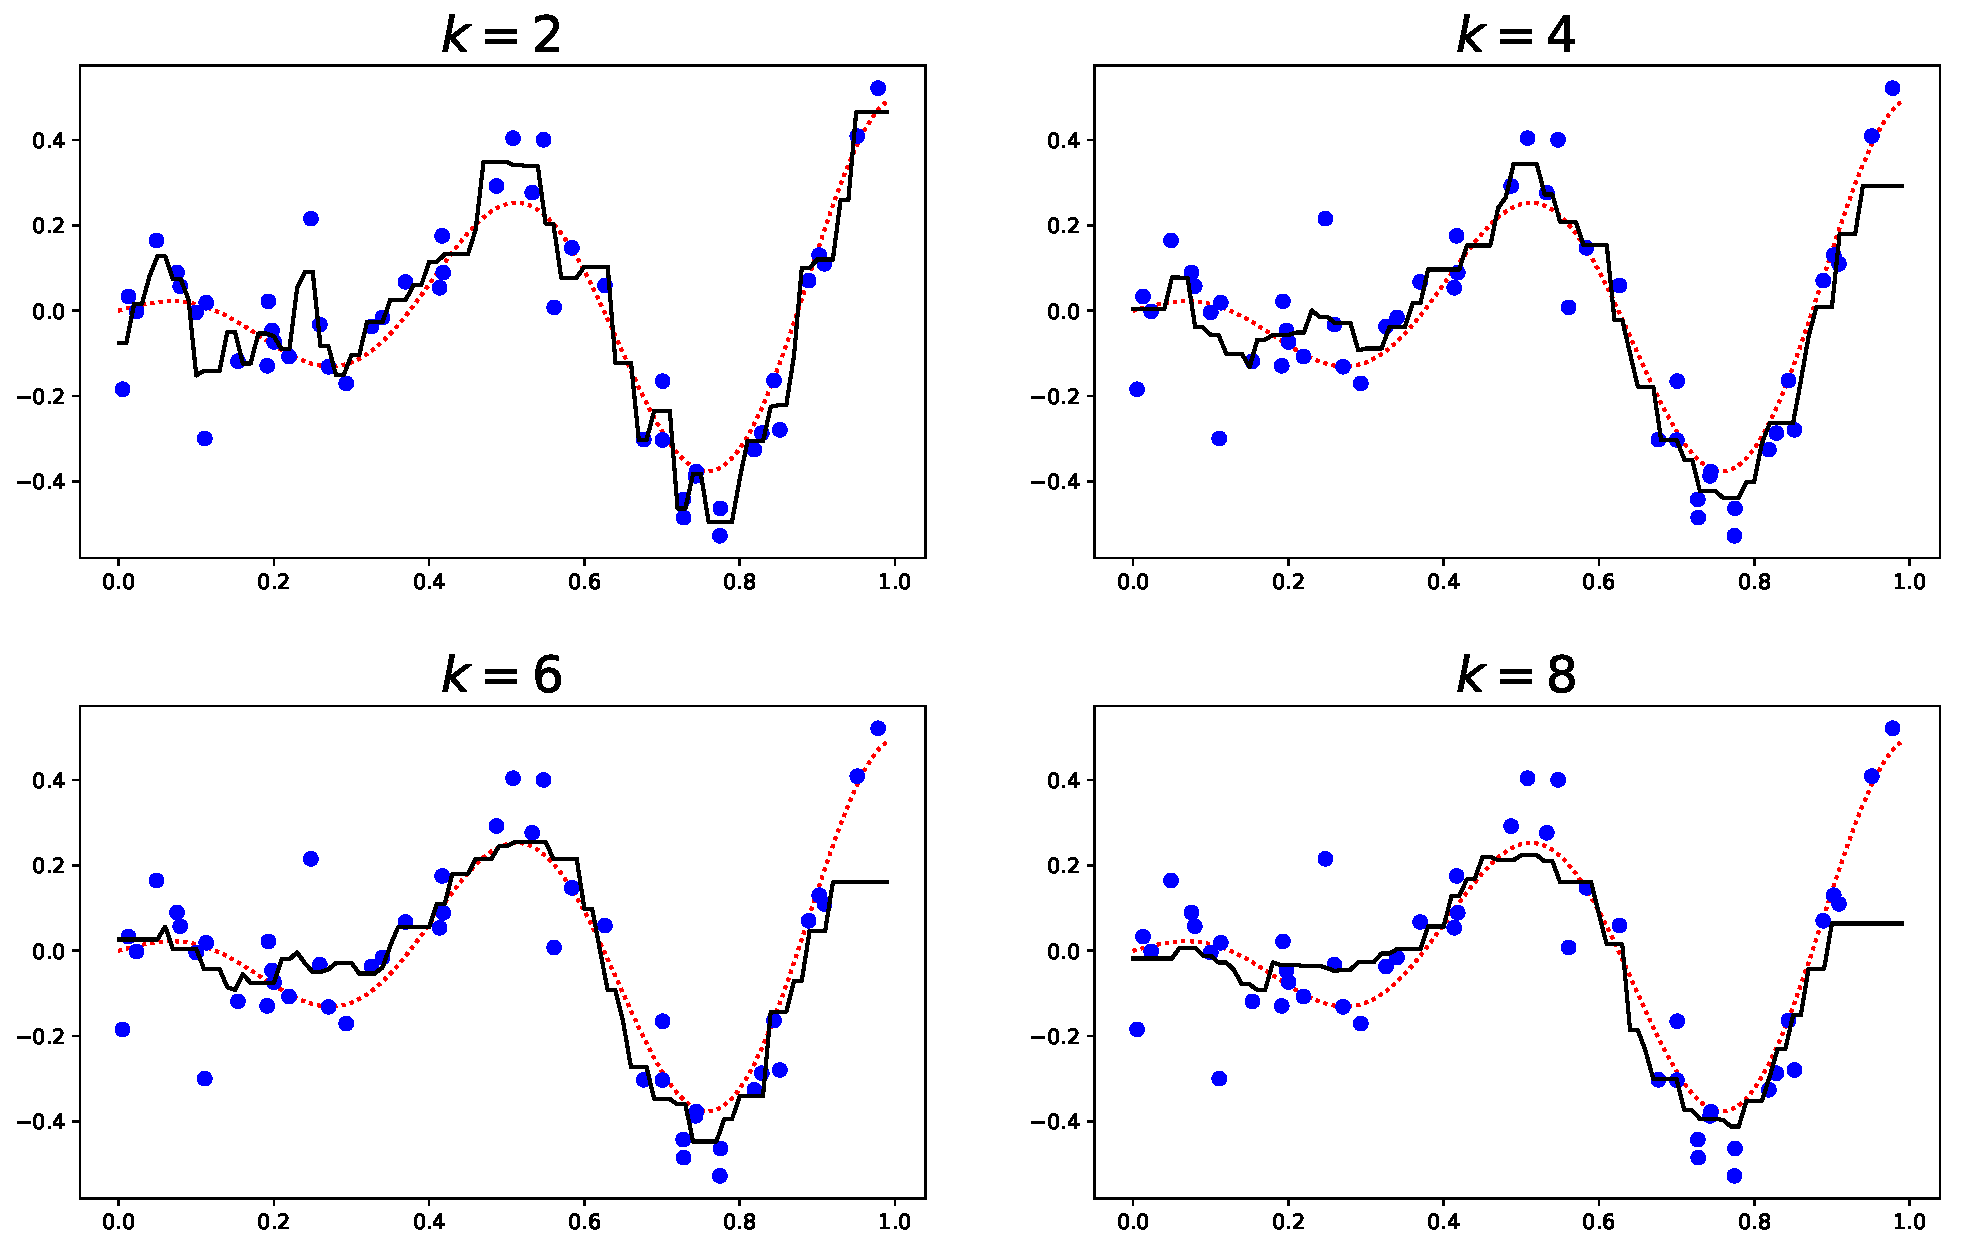
\includegraphics[scale=0.36]{knn_four_plots_1.pdf}
\end{frame}

\begin{frame}{}%{\textsc{$k$-nearest neighbors}}
    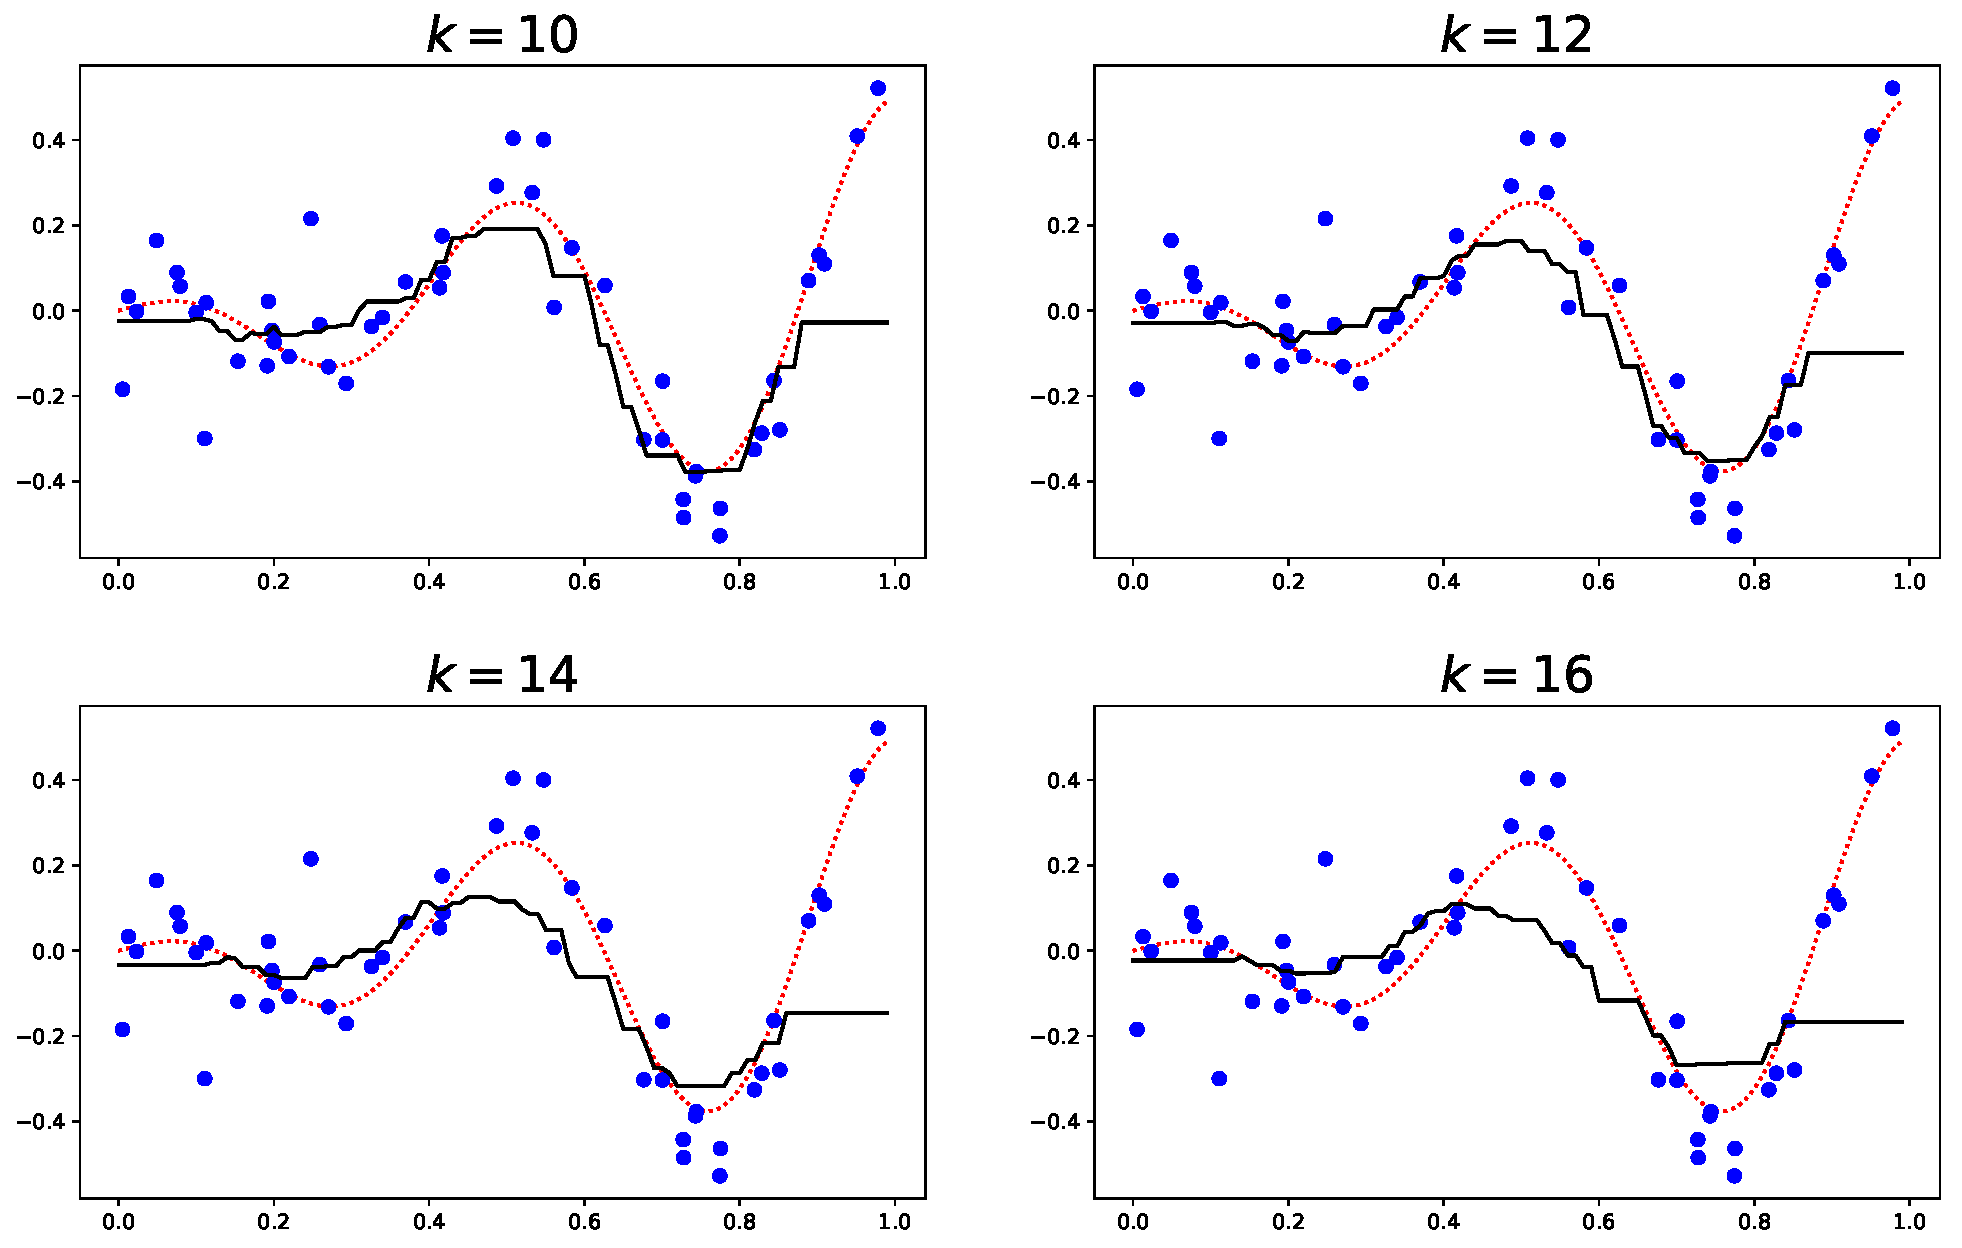
\includegraphics[scale=0.36]{knn_four_plots_2.pdf}
\end{frame}


\begin{frame}{\textsc{Example 2: Local averaging}}

\begin{block}{Definition}
    The \emph{local average smoother} with \emph{bandwidth $h>0$} is
    \[
        \hat r_h(\vx) = \frac{\sum_{\|\vx_i - \vx\|< h}Y_i}{\sum_{\|\vx_i - \vx\|< h}1}
    \]
    In words: $r_h(\vx)$ is the average of the $Y_i$ for which $\vx_i$
    lies a distance less than $h$ from $\vx$.
\end{block}
\end{frame}

\begin{frame}{}%{\textsc{$k$-nearest neighbors}}
    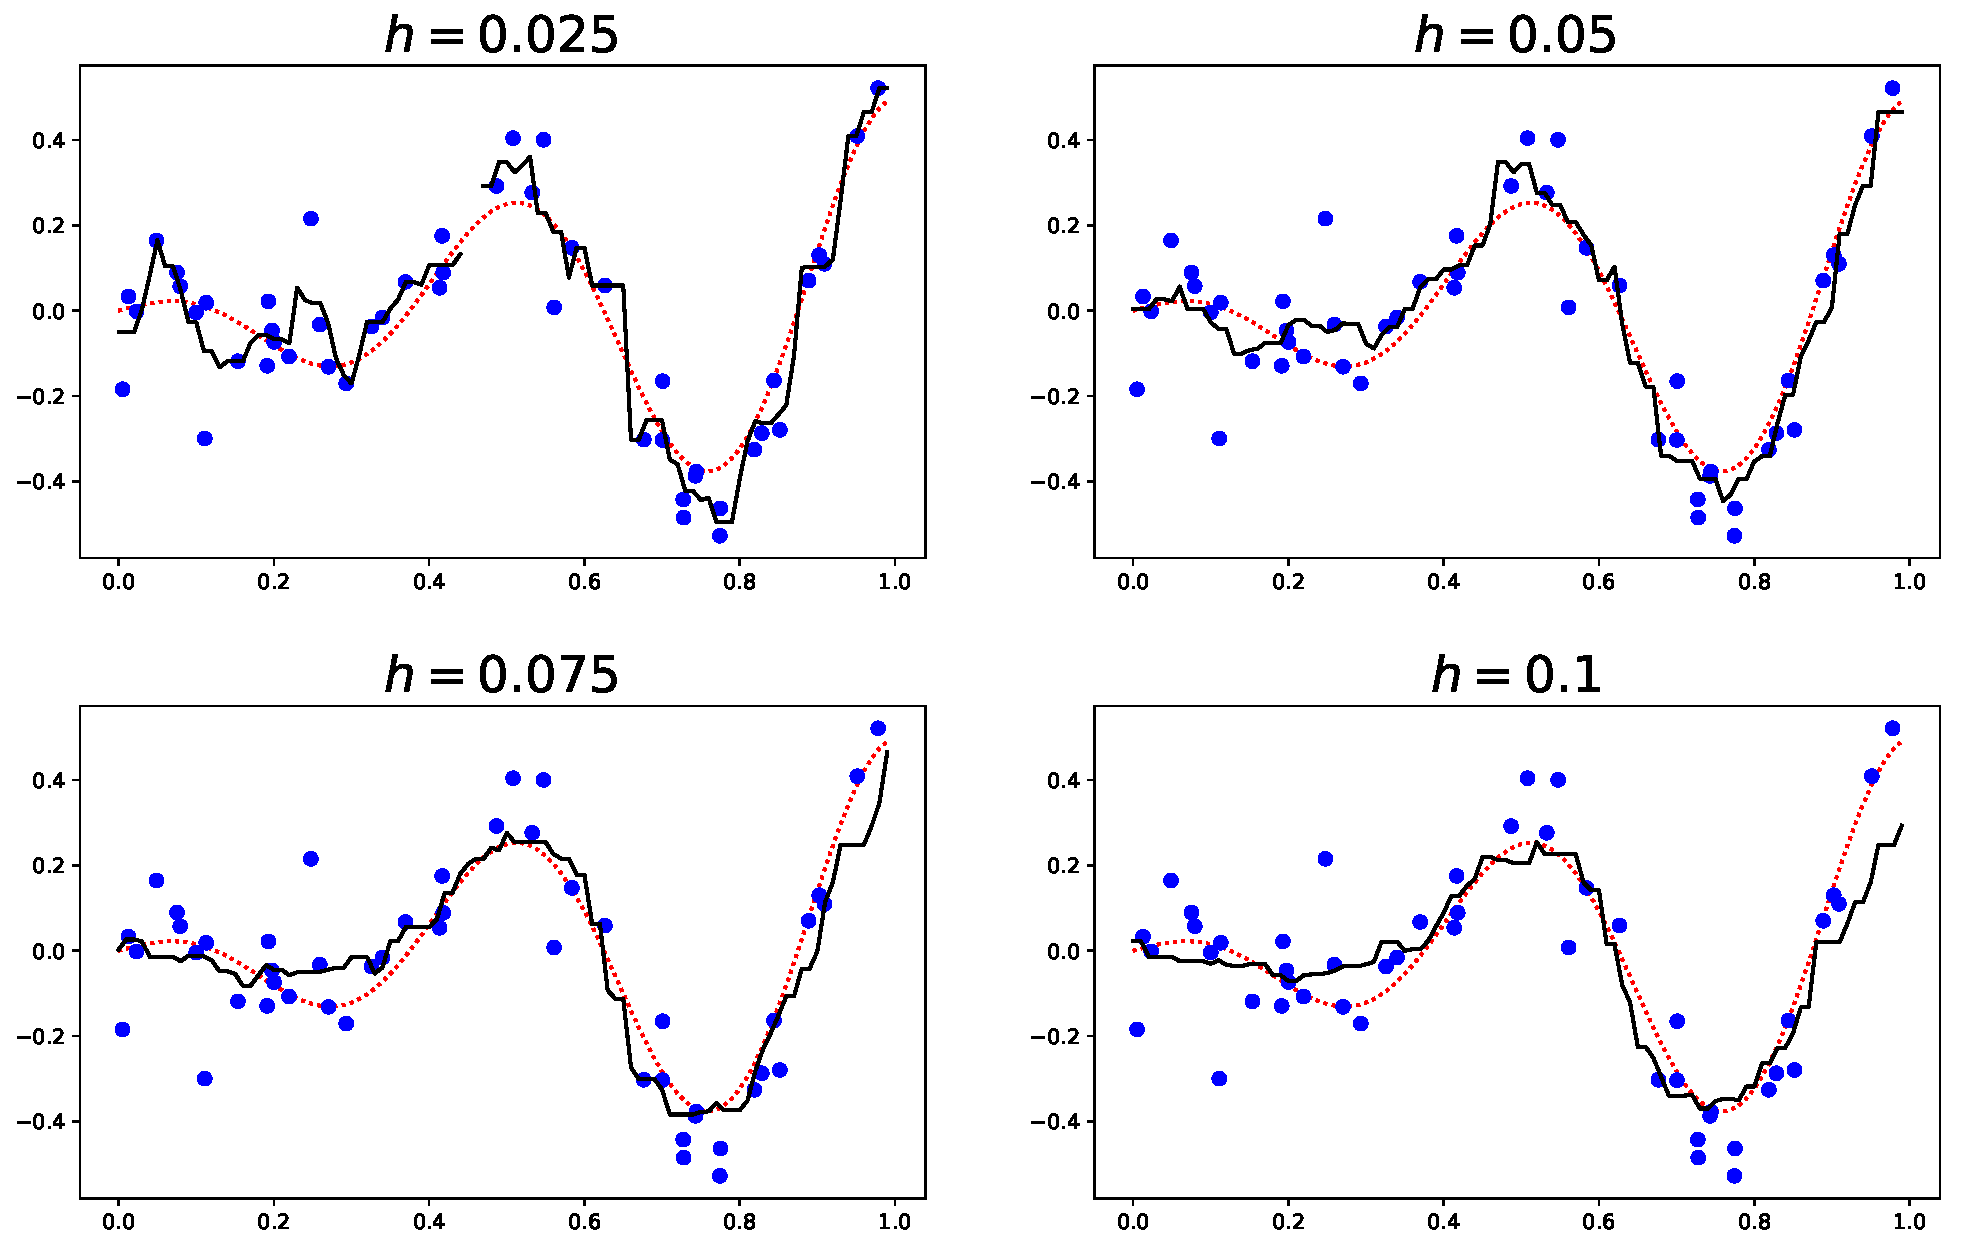
\includegraphics[scale=0.36]{la_four_plots_1.pdf}
\end{frame}

\begin{frame}{}%{\textsc{$k$-nearest neighbors}}
    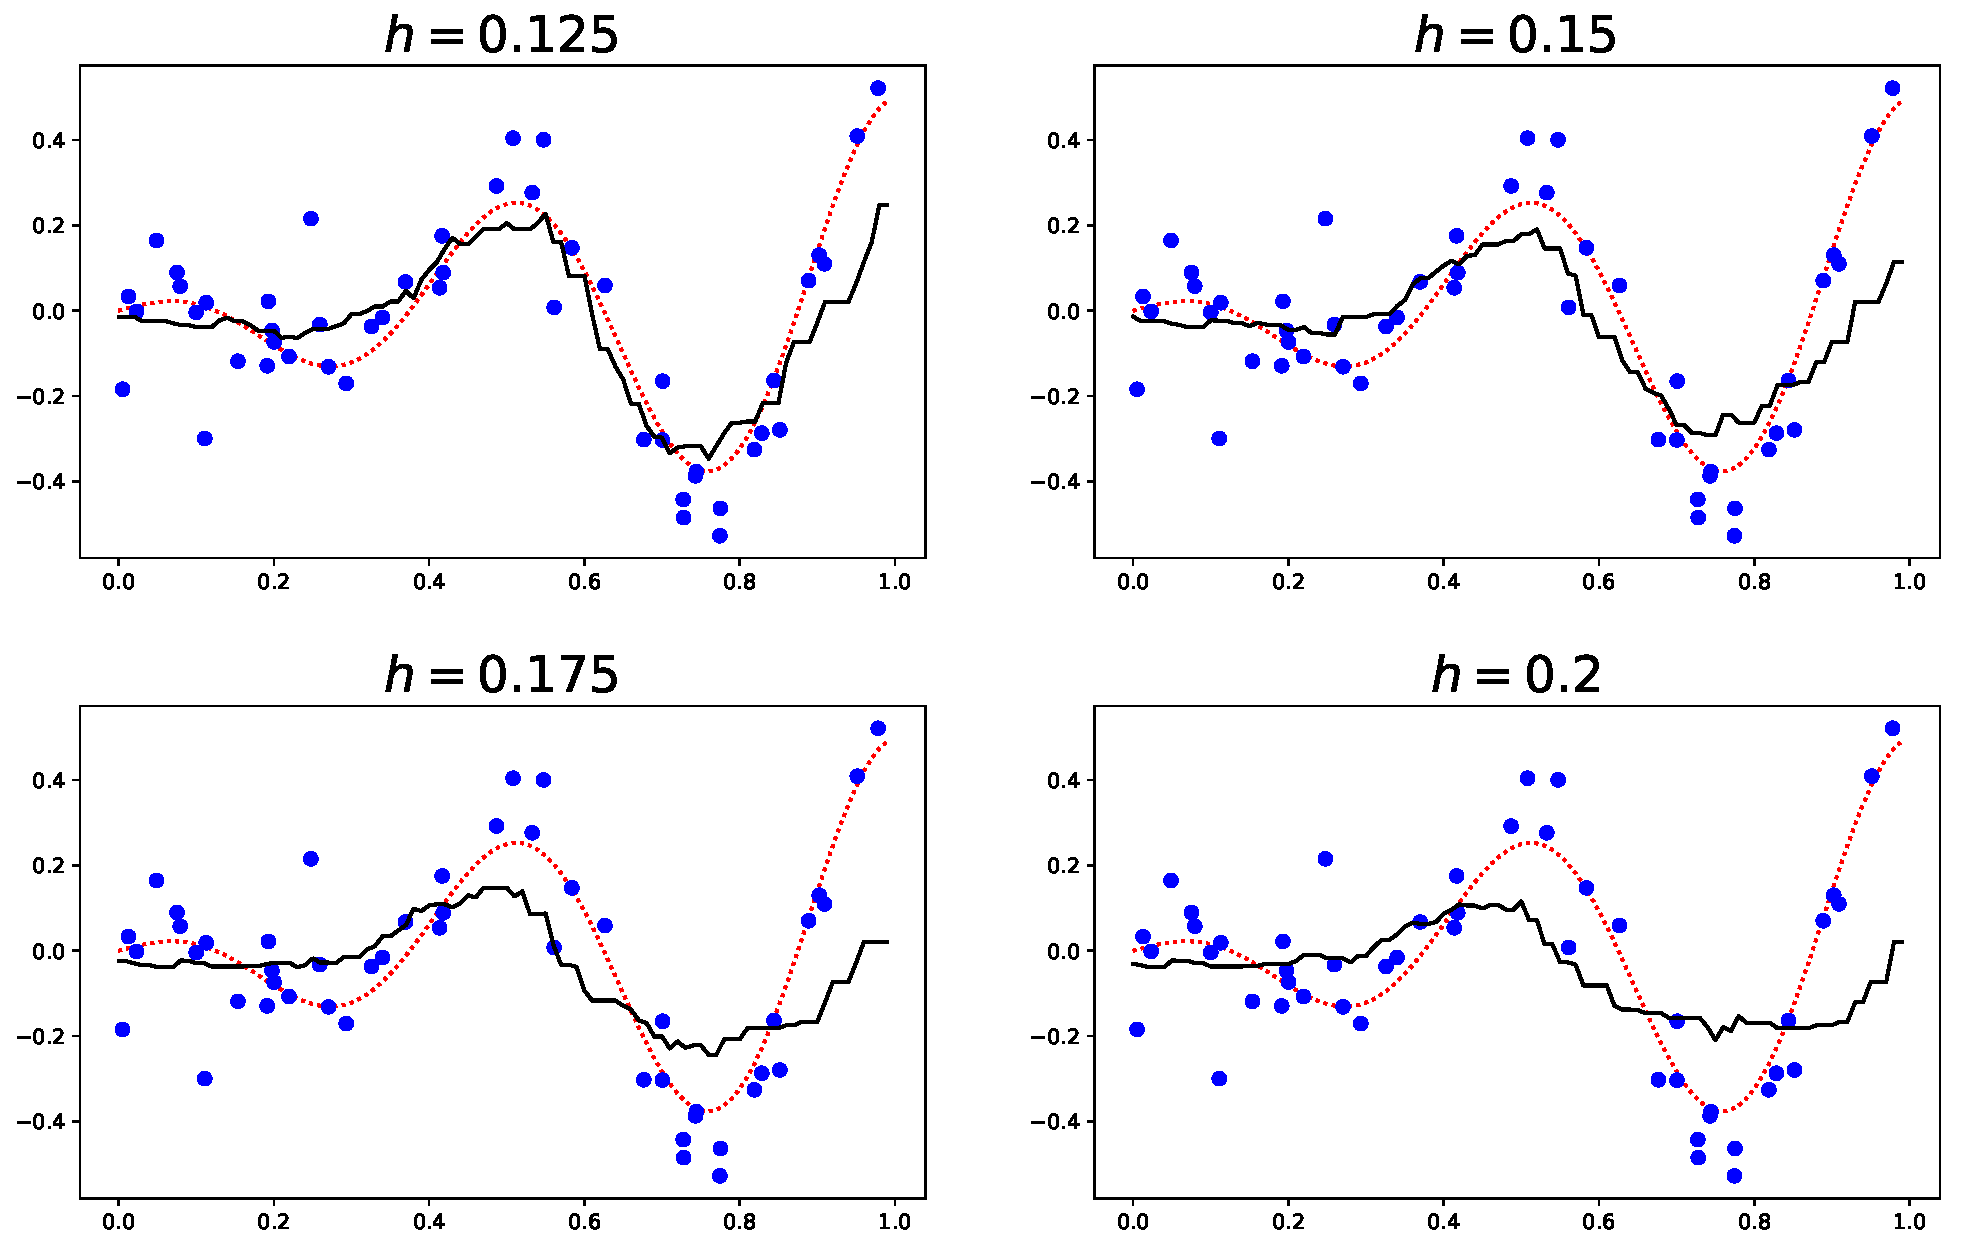
\includegraphics[scale=0.36]{la_four_plots_2.pdf}
\end{frame}

\begin{frame}{\textsc{Overfitting and Underfitting}}
    For small $k$ or $h$, the graphs of $\hat r(x)$ are too wiggly.
    We've \emph{overfit} or \emph{undersmoothed} the data.

    For big $k$ or $h$, the graphs of $\hat{r}(x)$ data very well (they're too flat).
    We say we've \emph{underfit} or \emph{oversmoothed} the data.

    How do we choose $k$ or $h$ optimally?
\end{frame}


\begin{frame}{\textsc{Evaluating smoothers: Loss and risk}}

    \begin{block}{Definitions}
        \begin{enumerate}\setlength\itemsep{1em}
            \item \emph{Squared error loss  at $x$:}
            \[
            L(\hat r(x), r(x)) := \big(\hat r(x) - r(x)\big)^2
        \]
        $\bullet$ $L(\hat r(x), r(x))$ is a random variable as $\hat r(x)$ is.

        \item \emph{Mean squared error (MSE)}  or \emph{risk} at $x$:
        \[
            R(\hat r(x), r(x)) := \EE\big[L\big(\hat r(x), r(x)\big)\big] 
            \approx \frac1n\sum_{i=1}^n L\big(\hat r(x_i), r(x_i)\big)
        \]

        \item \emph{Average MSE} or \emph{average risk}:
        \[
            R(\hat r, r) := \int R(\hat r(x), r(x))\,dx
            \approx \frac1n\sum_{i=1}^n R(\hat r(x_i), r(x_i))
        \]
        \end{enumerate}
    \end{block}
\end{frame}

\begin{frame}{\textsc{Choosing the smoothing parameter}}

    Obviously, smoothers with smaller average risk are preferred.

    So, choose the smoothing parameter to \emph{minimize average risk}:
    \[
        k := \argmin_k R(\hat r_k, r),\qquad
        h := \argmin_h R(\hat r_h, r)
    \]

    But there's a problem...
\end{frame}

\begin{frame}{\textsc{We don't know $r(x)$!}}
    \vspace{-5ex}
    \begin{align*}
        &\text{Loss at $x$:}& L(\hat r(x), r(x)) &= \big(\hat r(x) - r(x)\big)^2\\[2ex]
        &\text{Risk at at $x$:}& R(\hat r(x), r(x)) &= \EE\big[L\big(\hat r(x), r(x)\big)\big]\\[2ex]
            % &&&\approx \frac1n\sum_{i=1}^n L\big(\hat r(x_i), r(x_i)\big)\\[2ex]
        &\text{Average risk at at $x$:}& R(\hat r, r) &= \int R(\hat r(x), r(x))\,dx\\
        % &&&\approx \frac1n\sum_{i=1}^n R\big(\hat r(x_i), r(x_i)\big)\\[2ex]
    \end{align*}
    These expressions all involve $r(x)$, which we typically don't know!

    We can't compute these expressions; they also need to be estimated.
\end{frame}

\begin{frame}{\textsc{Coding activity 2}}
    \emph{But}, we can work in an artificial situation where we \emph{do} know $r(x)$:


    \begin{itemize}\setlength{\itemsep}{1ex}
        \item Choose:
        \begin{itemize}
            \item a function, $r(x)$
            \item $x_1,\ldots,x_n$
            \item a fine partition, $P$, of an interval containing the $x_i$
            \item $k$ (or $h$)
        \end{itemize}
            \item for $k=1,\ldots,K$
        \begin{itemize}
        \item for $j=0,\ldots,J-1$:
        \begin{itemize}
            \item Generate $y_i^{(j)}$, $1\leq i\leq n$, by sampling from $N(r_k(x_i), \sigma^2)$.
            \item Compute the losses $L(\hat r^{(j)}_k(x), r(x))$ at each $x$ in $P$.
        \end{itemize}
    \item Average the losses over $j$ to get the risks, $R(\hat r_k(x), r(x))$.
    \item Average the risks over $x$ to get the average risk, $R(\hat r_k, r)$.
    \end{itemize}
    \item Plot $R(\hat r_k, r)$ vs $k$ and choose $k$.
\end{itemize}
\end{frame}

\begin{frame}{\textsc{The bias-variance decomposition}}

    \begin{block}{Definition}
        The \emph{bias of $\hat r(x)$}, as an estimator of $r(x)$, is
        \[
            \Bias(\hat r(x), r(x)) := \EE[\hat r(x)] - r(x)
        \]
    \end{block}

    \begin{block}{Bias-variance decomposition}
        \[
            R(\hat r(x), r(x)) = \Var \hat r(x) + \Bias(\hat r(x), r(x))^2
        \]
    \end{block}

    \[
        \text{$\Var \hat r(x)$ big} \;/\; \text{graph of $\hat r$ wiggly} \;/\; \text{overfit}
        \;/\; \text{undersmoothed}
    \]
    \[
        \text{$\Bias(\hat r(x), r(x))$ big} \;/\; \text{graph of $\hat r$ too flat} \;/\; \text{underfit}
        \;/\; \text{oversmoothed}
    \]
\end{frame}

\begin{frame}{}
    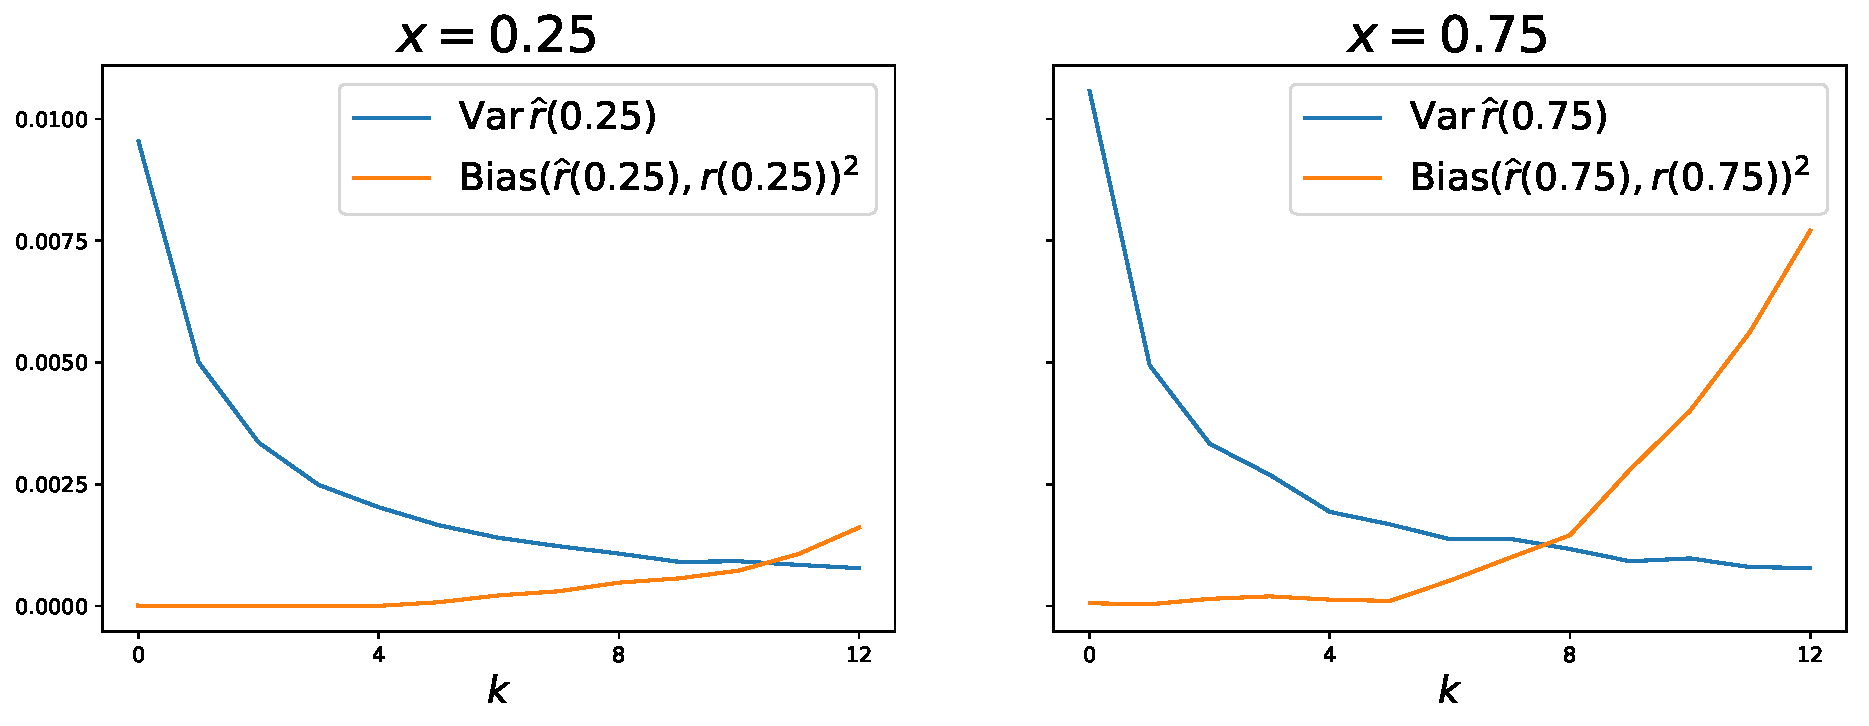
\includegraphics[scale=0.36]{bias_variance.pdf}

    Variance decreases as $k$ increases.

    Bias increases as $k$ increases.
\end{frame}

\begin{frame}{}
    Define:
    \[
        \Var \hat r := \int R(\hat r(x), r(x))\,dx,\qquad \Bias(\hat r, r)^2 := \int\Bias(\hat r(x), r(x))^2\,dx
    \]
    
    Integrate the bias-variance decomposition:
    \[
        R(\hat r, r) = \Var \hat r + \Bias(\hat r, r)^2
    \]

    Since $r$ is unknown, these quantities can only be estimated.
\end{frame}

\begin{frame}{\textsc{Coding activity 3}}
    \begin{itemize}
        \item For our running synthetic example, plot 
        \[
            R(\hat r_k, r),\; \Var \hat r_k,\; \text{and}\; \Bias(\hat r_k, r)^2
        \]
        versus $k$ on the same axes.

        \item Verify the integrated bias-variance decomposition using your computed
        $R(\hat r_k, r)$, $\Var \hat r_k$, and $\Bias(\hat r_k, r)^2$.
    \end{itemize}
     
    Reuse as much of your code from \textsc{coding activity 2} as possible.
\end{frame}

\begin{frame}{\textsc{Training error}}
    \begin{block}{Definition}
        The \emph{empirical risk} or \emph{training error} is
        \[
            \frac1n\sum_{i=1}^n L(\hat r(x_i), Y_i).
        \]
    \end{block}
    Empirical risk is not good estimator of $R$: We trained $\hat r$ on the 
    $(x_i,Y_i)$, making $L(\hat r(x_i), Y_i)$ biased downwards.
\end{frame}




\begin{frame}{\textsc{Leave one out cross-validation}}
    \begin{block}{Definition}
        The \emph{leave one out cross validation (LOOCV) score} is
        \[
            \hat R(h) := \frac1n\sum_{i=1}^n\big(Y_i - \hat r_h^{\,(-i)}(x_i)\big)^2,
        \]
        where $\hat r_h^{\,(-i)}$ is computed using the subdataset of the original one by removing the point $(x_i, Y_i)$.
    \end{block}
    \vspace{-1ex}$\hat R(h)$ is typically a good estimator of the average risk of $\hat r_h$:
    \[
        \hat R(h) \approx R(\hat r_h, r) + \sigma^2,\quad\text{where}\quad\sigma^2 = \Var Y_i.
    \]
    We choose our smoothing parameter to be the one that minimizes $\hat R(h)$:
    \[
        h := \argmin_h \hat R(h)
    \]
\end{frame}

\begin{frame}{\textsc{Coding activity 4}}
    For our running example, plot $\hat R(k)$ versus $k$. Compute the $\hat R(k)$ using
    \texttt{sklearn}'s \texttt{LeaveOneOut} class and the generator returned by its
    \texttt{split} method.
    
    Which $k$ that minimizes $\hat R(k)$? Compare with the results of \textsc{coding activity 2}.

    For this optimal value of $k$, plot $\hat r_k^{(-i)}(x_i)$ versus $x_i$ and $r(x)$ versus $x$ on the same axes.

    \textit{Remark:} \texttt{LeaveOneOut} is fairly low-level; \texttt{sklearn} provides more 
    convenient ways to tune hyperparameters using cross validation.
    Sometimes, though, it's necessary to work with the lower-level constructs.
\end{frame}

\begin{frame}{\textsc{$K$-fold cross validation}}
Partition $\{1,\ldots,n\}$ into $K$ \emph{folds}, $I_1,\ldots,I_K$, of roughly equal size.

Let $\hat r_h^{(-I_j)}$ be the smoother computed using the subdataset of the original one
obtained by removing $(x_i, Y_i)$, for $i\in I_j$.

\begin{block}{Definition}
    The \emph{$K$-fold cross validation score is}
    \[
        \hat{R}_K(h) := \sum_{j=1}^K\frac1{|I_j|}\sum_{i\in I_j}\big(Y_i - r_h^{(-I_j)}(x_i)\big)^2
    \]
\end{block}

We can use $\hat{R}_K$ in place of $\hat{R}$ to select a smoothing parameter.

In practice, $K$ is usually $5$ (\texttt{sklearn}'s default) or $10$.
\end{frame}

\begin{frame}{\textsc{Coding activity 5}}
    Find the values of $k$ that minimnize the $3$-, $5$-, and $10$-fold cross validation scores.
    Compute these scores using \texttt{cross\_val\_score} from \texttt{sklearn.model\_selection}.
    
    Confirm your results from \textsc{coding activity 4} by performing LOOCV as 
    $n$-fold cross validation, $n$ being the size of the dataset.
\end{frame}

\end{document}